\documentclass[12pt]{cornouaille}
\dscornouaille



\begin{document}






:::exercice Exercice 1: Pour les candidats ayant suivi l'enseignement de spécialité /5 points




On s'intéresse à la figure suivante, dans laquelle $a$, $b$ et $c$ désignent les longueurs des hypoténuses des trois triangles rectangles en O dessinés ci-dessous.



\psset{unit=3cm}

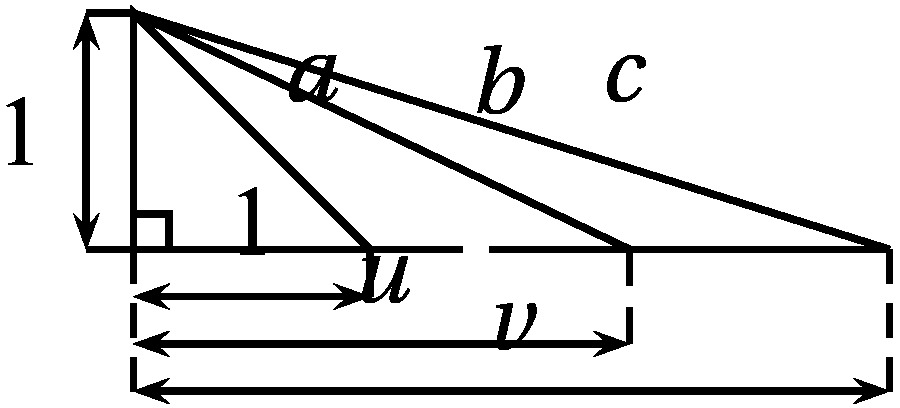
\includegraphics{./TS-BacBlanc-2020-Spe-0}




\textbf{Problème :} on cherche les couples de \textbf{nombres entiers naturels non nuls} $(u,~v)$ tels que $ab = c$.

\medskip





\textbf{1. } Modélisation

Démontrer que les solutions du problème sont des solutions de l'équation :


$$
(E) :\quad  v^2 - 2u^2 = 1\quad  (v \text{ et }\: u \: \text{ étant des entiers naturels non nuls}).
$$


:::startsolution

Dans le triangle rectangle, on applique le théorème de
Pythagore : $a^2=1^2+1^2=2$.

En appliquant le théorème dans les deux autres triangles rectangles on
peut écrire :

$b^2=1^2+u^2=1+u^2$ et $c^2=1^2+v^2=1+v^2$.

$a$, $b$ et $c$ sont 3 longueurs donc sont des nombres positifs donc
$ab=c \iff a^2b^2=c^2$; ainsi $2(1+u^2)=1+v^2$ c'est-à-dire
$2+2u^2=1+v^2$ donc $v^2-2u^2=1$.

Les solutions du problème sont donc les solutions $(u~;~v)$ de l'équation
$(E): \, v^2 - 2u^2=1$ où $u$ et $v $ sont des entiers naturels non nuls.


:::endsolution



\textbf{2. }  Recherche systématique de solutions de l'équation $(E)$

Recopier et compléter l'algorithme suivant pour qu'il affiche au cours de son exécution tous les couples solutions de l'équation pour lesquels $1 \leqslant u \leqslant 1000$ et $1 \leqslant v \leqslant 1000$.




\begin{tabularx}{\linewidth}{|X|m{4.5cm}|}\hline
Pour $u$ allant de 1 à \ldots faire&Au cours de son exécution,\\
\hspace{0.5cm}Pour \ldots&l'algorithme affiche :\\
\hspace{1cm}Si \ldots&2 \quad 3\\
\hspace{1.5cm}Afficher $u$ et $v$&12 \quad 17\\
\hspace{1cm}Fin Si&70 \quad 99\\
\hspace{0.5cm}Fin Pour&408 \quad 577\\
Fin Pour&\\ \hline
\end{tabularx}




:::startsolution

Algorithme :




\begin{tabularx}{\linewidth}{|X|m{4.5cm}|}\hline
Pour $u$ allant de 1 à 1000 faire&Au cours de son exécution,\\
\hspace{0.5cm}Pour $v$ allant de 1 à 1000 &l'algorithme affiche :\\
\hspace{1cm}Si $v^2-2u^2=1$&2 \quad 3\\ \cdashline{2-2}
\hspace{1.5cm}Afficher $u$ et $v$&12 \quad 17\\ \cdashline{2-2}
\hspace{1cm}Fin Si&70 \quad 99\\ \cdashline{2-2}
\hspace{0.5cm}Fin Pour&408 \quad 577\\
Fin Pour&\\ \hline
\end{tabularx}




:::endsolution



\textbf{3. } Analyse des solutions éventuelles de l'équation $(E)$

On suppose que le couple $(u,~v)$ est une solution de l'équation $(E)$.




\textbf{3.a) } Établir que $u < v$.


:::startsolution

Supposons que le couple $(u,v)$ est une solution de l'équation $(E)$ et que $u\geqslant v$.

On a alors :  $u^2 \geqslant v^2$ et comme $2u^2 \geqslant u^2$, on a $2u^2 \geqslant v^2$ ce qui implique $v^2-2u^2\leqslant 0$.

C'est impossible car $v^2-2u^2=1$.

Conclusion : $u < v$.


:::endsolution


\textbf{3.b) }  Démontrer que $n$ et $n^2$ ont la même parité pour tout entier naturel $n$.


:::startsolution

On suppose que $n$ est pair. Il existe alors un entier naturel $k$
tel que $n=2k$.

On a alors $n^2=(2k)^2=4k^2=2(2k^2)$. Ainsi $n^2$ est pair.

On suppose que $n$ est impair. Il existe alors une entier naturel $q$ tel
que $n=2q+1$.

Alors $n^2=(q+1)2=4q^2+4q+1=2(2q^2+2q)+1$. Ainsi  $n^2$ est impair.


Conclusion : $n$ et $n^2$ ont la même parité.


:::endsolution



\textbf{3.c) }  Démontrer que $v$ est un nombre impair.


:::startsolution

Soit un couple solution $(u,v)$ du problème. On a  :

$v^2-2u^2=1 \iff v^2=2u^2+1$.

Ainsi $v^2$ est impair. D'après la question précédente $v$ est aussi impair.


:::endsolution


\textbf{3.d) }  Établir que $2u^2 =(v-1)(v+1)$.

En déduire que $u$ est un nombre pair.


:::startsolution

On a : $v^2-2u^2=1 \iff 2u^2=v^2-1 \iff 2u^2=(v-1)(v+1)$.

Or $v$ est impair donc $v-1$ et  $v+1$ sont pairs : il existe ainsi un
entier naturel $k$ tel que $v-1=2k$ et $v+1=2(k+1)$.

Alors $2u^2=2k \times 2(k+1) \iff u^2=2k(k+1)$.

$u^2$ est donc pair. D'après la question \textbf{3.b.}, $u$ est donc pair.


:::endsolution




\textbf{4. }  Une famille de solutions

On assimile un couple de nombres entiers $(u,~v)$ à la matrice colonne $X = 
\begin{pmatrix}u\\v\end{pmatrix}
$.

On définit également la matrice $A = 
\begin{pmatrix}3&2\\4&3\end{pmatrix}
$.




\textbf{4.a) } Démontrer que si une matrice colonne $X$ est une solution de l'équation $(E)$, alors $AX$ est aussi une solution de l'équation $(E)$.


:::startsolution

Soit $X=
\begin{pmatrix}		u\\v		\end{pmatrix}
$ une solution de l'équation $(E)$.

$AX=
\begin{pmatrix} 3&2\\ 4&3 \end{pmatrix}
 \times 
\begin{pmatrix} u\\ v
\end{pmatrix}
=
\begin{pmatrix} 3u+2v\\ 4u+3v\end{pmatrix}
$.

On a : $(4u+3v)^2-2(3u+2v)^2=16u^2+24uv+9v^2-18u^2-24uv-8v^2=v^2-2u^2=1$.

Ainsi $AX$ est aussi solution de $(E)$.


:::endsolution


\textbf{4.b) } Démontrer que si une matrice colonne $X$ est une solution de l'équation $(E)$, alors pour tout entier naturel $n$,\: $A^n X$ est aussi une solution de l'équation $(E)$.


:::startsolution

Montrons par récurrence que pour tout entier naturel $n$, $A^nX$ est une solution de l'équation $(E)$.


\begin{itemize}
\item Initialisation : $n=0$.

$A^0X=I_2X=X$. Et $X$ est solution de $(E)$. L'affirmation est donc vraie pour $n=0$.

\item Soit $n \geqslant 0$ quelconque tel que $A^nX$ est une solution de $(E)$.

$A^{n+1}X=A \times A^nX$ est une solution de $(E)$ d'après la question précédente.
\item Conclusion : la propriété est vraie pour $n=0$ et est
héréditaire pour tout $n\geqslant 0$. D'après le raisonnement par récurrence, la propriété est vraie pour tout $n\geqslant 0$.
\end{itemize}


On a donc démontré que, si $X$ est une solution de $(E)$, alors, pour tout entier naturel $n$, $A^nX$ est aussi une solution de $(E)$.


:::endsolution


\textbf{4.c) } À l'aide de la calculatrice, donner un couple $(u,~v)$ solution de l'équation $(E)$ tel que

$v > 10000$.


:::startsolution

On a : $3^2-2 \times 2^2=9-8=1$ donc le couple $(2;3)$ est solution de $(E)$.

$A^5 \times X = 
\begin{pmatrix} 13860\\ 19601\end{pmatrix}
$.

Donc le couple $(13860~;~19601)$ est une solution de $(E)$ telle que $v > 10000$.


:::endsolution








:::




\end{document}